\chapter{软件分布式共享内存JIAJIA系统简介}\label{chap:JIAJIA}{
    JIAJIA 是一个国产软件 DSM 系统,本身主要基于共享内存系统技术与UDP技术搭建而成,
    以页为共享粒度,在物理分离的内存上提供逻辑共享的虚拟内存。
    系统以用户库的形式提供给开发人员,开发人员可以使用 jia.h 头文件提供的接口编写采用分布式共享内存范式的并行程序,
    并使用 .jiahosts 配置文件设置参与分布式系统的节点组成,本文的主要工作也在JIAJIA系统上开展。

    \section{软件分布式共享内存系统 JIAJIA}
    \subsection{设计架构}
    % \begin{figure}[!htbp]
    %     \centering
    %     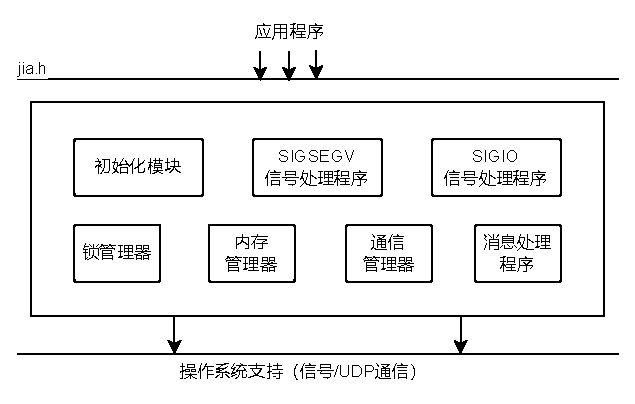
\includegraphics[width=\textwidth]{Img/JIAJIA 设计架构.drawio.pdf}
    %     \bicaption{\enspace JIAJIA 设计架构}{\enspace JIAJIA design architecture}
    %     \label{fig:JIAJIA-design}
    % \end{figure}

    程序运行时,JIAJIA系统将会拷贝应用程序和配置文件到所有参与节点,随后并行执行协同完成任务。

    \begin{enumerate}[label=\arabic*.]
        \item \textbf{初始化模块。}初始化模块用于对整个系统进行准备操作,负责加载配置文件(.jiahosts,.jiaconfig)以及初始化各个模块。
              %   \begin{figure}[!htbp]
              %       \centering
              %       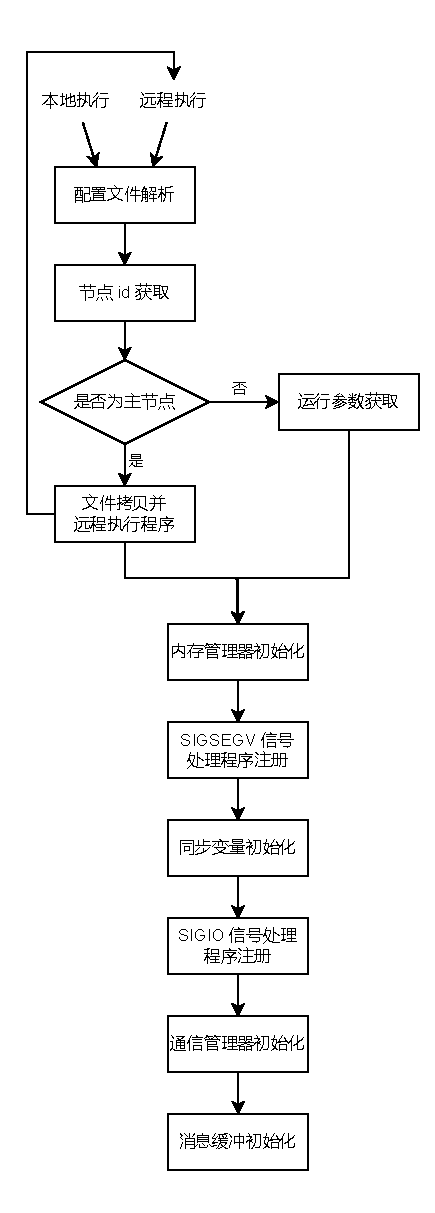
\includegraphics[width=0.6\textwidth]{Img/JIAJIA初始化模块.drawio.pdf}
              %       \bicaption{\enspace JIAJIA 初始化模块}{\enspace JIAJIA initialization module}
              %       \label{fig:JIAJIA-init}
              %   \end{figure}

        \item \textbf{内存管理器。} JIAJIA 采用 NUMA 结构,是一个基于宿主(home-based)的系统,每个共享页都有对应的宿主节点核心包含三个数据结构:用于记录本地分配的共享页的目录(home),用于记录缓存页状态的缓存目录(cache),用于记录全部共享页的页目录(page)。JIAJIA 的内存组织如~\ref{fig:JIAJIA-memory}所示。
              \begin{figure}[!htbp]
                  \centering
                  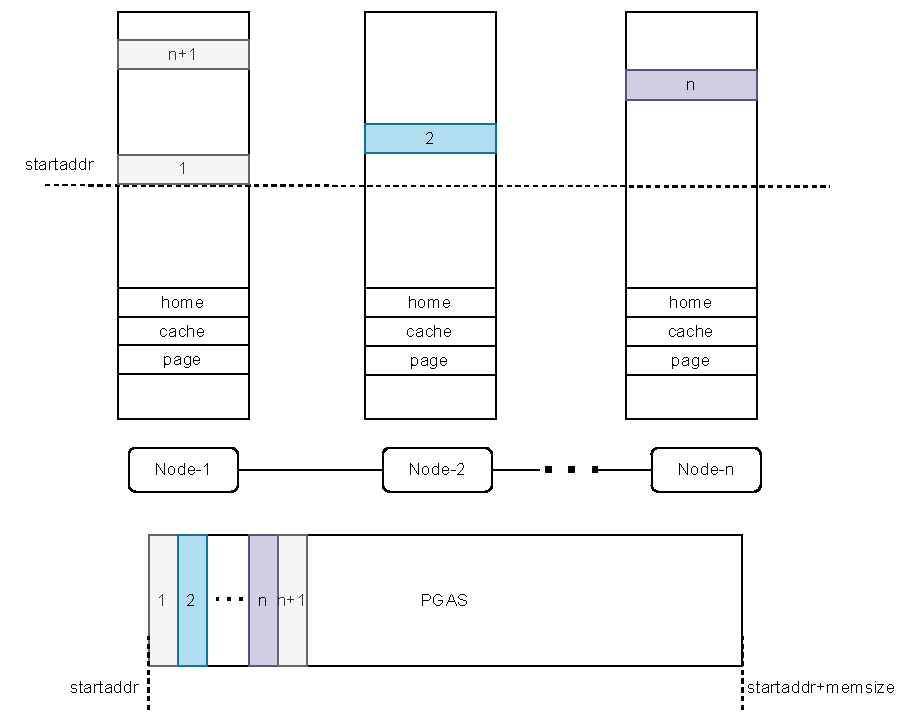
\includegraphics[width=0.86\textwidth]{Img/JIAJIA内存组织.drawio.pdf}
                  \bicaption{\enspace JIAJIA 内存组织}{\enspace JIAJIA memory structure}
                  \label{fig:JIAJIA-memory}
              \end{figure}

        \item \textbf{SIGSEGV 信号处理程序。} JIAJIA 系统中任何节点都可以透明地访问任一共享内存位置。这一机理利用了操作系统的信号机制:当应用程序试图访问无权限内存时,将触发段违例信号(SIGSEGV),操作系统将捕获该信号并将其发送给预设的 SIGSEGV 信号处理程序。该程序将完成对本地内存的授权或对远程内存的取页操作。如图~\ref{fig:JIAJIA-access}所示。
              \begin{figure}[!htbp]
                  \centering
                  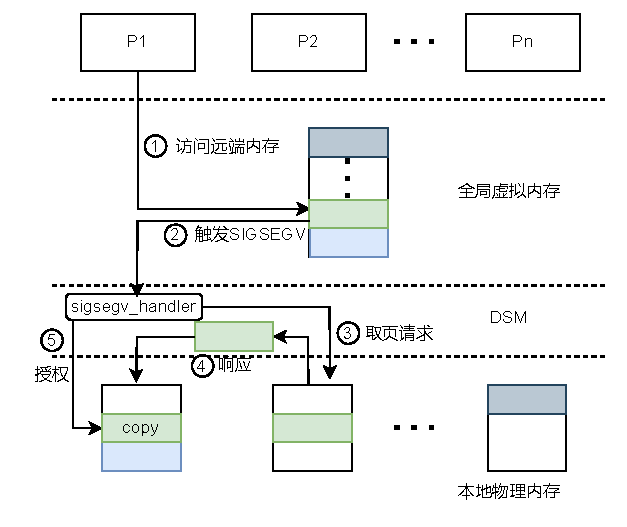
\includegraphics[width=0.68\textwidth]{Img/JIAJIA访问远端内存.drawio.pdf}
                  \bicaption{\enspace JIAJIA 访问远端内存}{\enspace JIAJIA }
                  \label{fig:JIAJIA-access}
              \end{figure}

        \item \textbf{通信管理器。} JIAJIA 使用通信管理器记录并管理发送和接收的套接字描述符。

              \begin{figure}[!htbp]
                  \centering
                  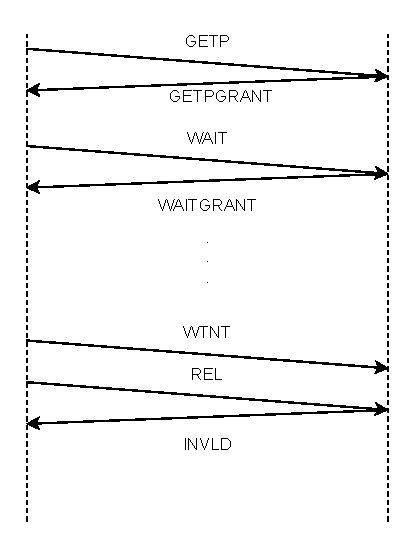
\includegraphics[width=0.4\textwidth]{Img/JIAJIA底层消息传递机制.drawio.pdf}
                  \bicaption{\enspace JIAJIA 底层消息传递机制}{\enspace JIAJIA underlying message passing mechanism}
                  \label{fig:JIAJIA-message-handle}
              \end{figure}
        \item \textbf{消息处理程序。} JIAJIA 底层基于消息传递机制,消息处理程序主要负责处理接收到的本地或远程消息,并根据消息类型执行相应的操作。
              如图~\ref{fig:JIAJIA-message-handle}。


              %   \begin{figure}[!htbp]
              %       \centering
              %       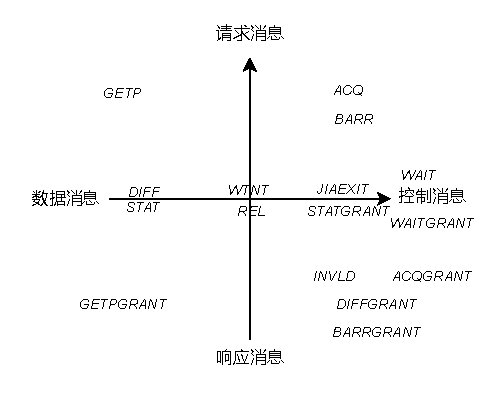
\includegraphics[width=0.7\textwidth]{Img/JIAJIA消息类型.drawio.pdf}
              %       \bicaption{\enspace JIAJIA 消息类型}{\enspace JIAJIA message types}
              %       \label{fig:JIAJIA-message-types}
              %   \end{figure}

        \item \textbf{锁管理器。}
              锁管理器主要负责同步变量的分配管理,如图~\ref{fig:JIAJIA-lock-manager}。JIAJIA 支持两种同步变量:锁(lock)和屏障(barrier),处理方式如下:
              \begin{itemize}
                  \item 对于锁同步变量,锁管理器维护一个先入先出队(FIFO)队列,按请求顺序依次授予锁权限;
                  \item 对于屏障同步变量,锁管理器通过计数器判断所有节点是否抵达相同位置,并在全部到达后统一授予继续运行的权限
              \end{itemize}
              \begin{figure}[!htbp]
                  \centering
                  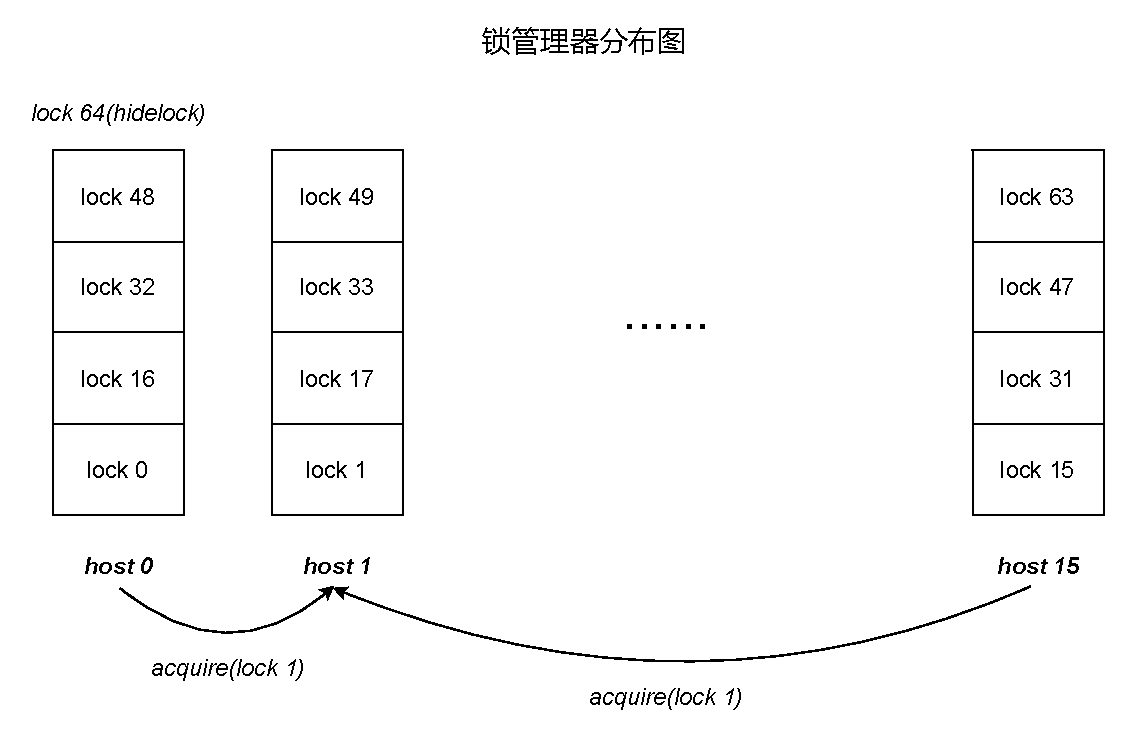
\includegraphics[width=1.0\textwidth]{Img/JIAJIA锁管理器.drawio.pdf}
                  \bicaption{\enspace JIAJIA 锁管理器分布}{\enspace JIAJIA lock-managers layout}
                  \label{fig:JIAJIA-lock-manager}
              \end{figure}
    \end{enumerate}

    % \newpage
    \subsection{基于锁的缓存一致性协议}
    在内存一致性模型方面,JIAJIA 采用域一致性模型,并实现了一种基于锁的缓存一致性协议。该协议支持写失效的传播策略,并利用多写协议来避免假共享。

    JIAJIA 使用同步变量将应用程序分割为一个个一致性域(或称为临界区间),每到达一个同步原语都代表一个旧临界区间的结束,以及新临界区间的开始。
    每次在一个临界区间(如scope1)结束时,将传播在该临界区中对共享页做的修改给相应的宿主节点。

    JIAJIA 基于锁的一致性协议的特点是它将一个临界区域内对共享页的修改信息(写通知,write-notice)与锁绑定,
    write-notice 记录了修改页的地址(见图~\ref{fig:JIAJIA-lockstack}),获取锁的处理机将根据锁管理器中的 write-notice 得知哪些页面已被其他处理机修改。
    在处理临界区嵌套情况时,JIAJIA 使用堆栈结构来记录锁的嵌套,获取锁时压栈,释放锁时弹栈,
    弹栈时将把栈顶锁的 write-notice 合并到下一层,同时把栈顶的write-notice发送给对应的锁管理器。

    \begin{figure}[!htbp]
        \centering
        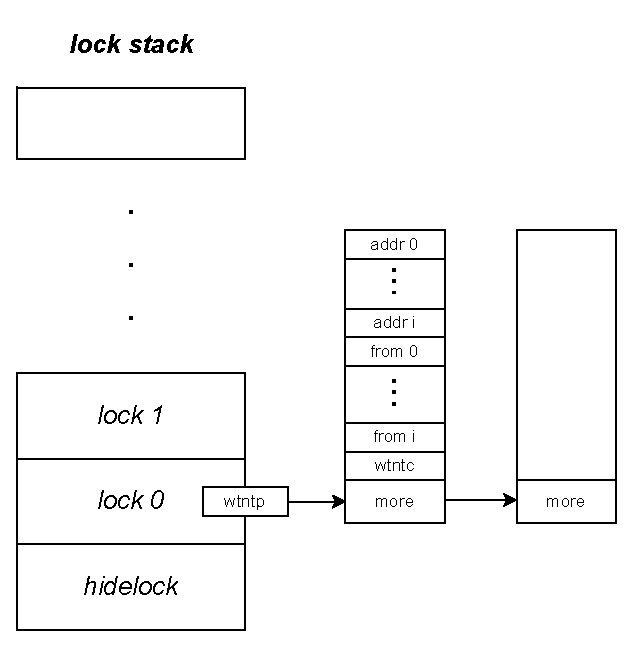
\includegraphics[width=0.6\textwidth]{Img/JIAJIA锁栈结构.drawio.pdf}
        \bicaption{\enspace JIAJIA 锁栈结构}{\enspace JIAJIA lockstack layout}
        \label{fig:JIAJIA-lockstack}
    \end{figure}

    每当JIAJIA系统进行同步操作时,主机会将当前临界区修改的地址对应的write-notice信息记录到当前栈顶的锁上,
    并将修改的内容发送到对应的主机上(修改home节点内容)。
    jia\_unlock或jia\_barrier操作时,主机会在弹栈的同时将栈顶锁的write-notice发送给对应的锁管理器,方便其他主机同步;
    jia\_lock或jia\_barrier操作时,主机也会从对应的锁管理器拿到相应的write-notice信息,并将本地的对应的页面无效化。

    以jia\_barrier为例,下图是jia\_barrier时同步操作的流程:

    % \begin{figure}[!htbp]
    %     \centering
    %     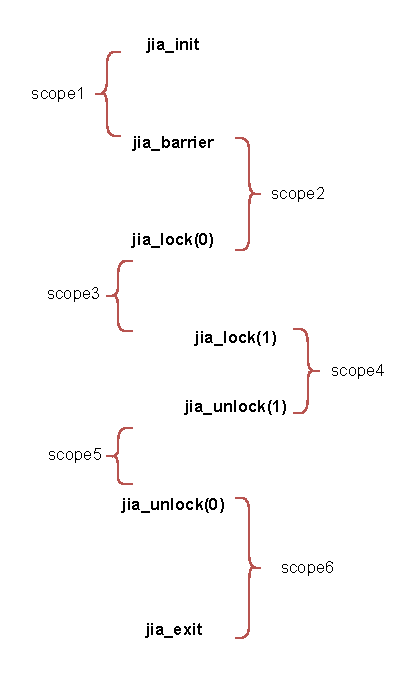
\includegraphics[width=0.60\textwidth]{Img/JIAJIA一致性域.drawio.pdf}
    %     \bicaption{\enspace JIAJIA 一致性域}{\enspace JIAJIA consistency scope}
    %     \label{fig:JIAJIA-scopes}
    % \end{figure}

    % \begin{figure}[!htbp]
    %     \centering
    %     \includegraphics[width=0.1\textwidth]{Img/jiajia_barr_sync.drawio.pdf}
    %     \bicaption{\enspace JIAJIA 锁栈结构}{\enspace JIAJIA lockstack layout}
    %     \label{fig:JIAJIA-lockstack}
    % \end{figure}

    假设初始状态是(host1为local主机,图中红色(黄色)代表了对某一个页面的一种修改,白色代表没有修改):
    \begin{itemize}
        \item page1: home节点在host1,主机2与主机3修改,远程有备份;
        \item page2: home节点在host1,主机1修改,远程有备份;
        \item page3: home节点在host2,主机1修改,,远程有备份;
    \end{itemize}
    \begin{enumerate}[label=\arabic*.]
        \item senddiffs操作时,若远程主机修改了页面(即不为该页面的home主机),将会计算本地修改的内容,并将diff消息打包后发送给home主机进行处理更新。
              如果有两台主机进行了修改,则发送的先后顺序是不确定的。若要求有确定的执行顺序,
              需要由编程人员保证同一临界区间内同一页面只有一台主机进行了修改。(图~\ref{fig:JIAJIA-barrier1})
        \item sendwtnts操作时,每台主机将本地锁栈顶端锁记录的wtnts发送给对应的锁管理器。对于barrier的情况,将有hidelock(64号锁)担任此角色。
              对应的锁管理器,如果在发送过来的wtnts中发现对某一页面有不同主机的修改,则记录frompid为Maxhosts,
              否则记录为对应的主机。(图~\ref{fig:JIAJIA-barrier1})

              \newpage
              \begin{figure}[!htbp]
                  \centering
                  \includegraphics[width=0.8\textwidth,page=1]{Img/jiajia_barr_sync.drawio.pdf}
                  \bicaption{\enspace JIAJIA barrier同步操作}{\enspace JIAJIA barrier sync1}
                  \label{fig:JIAJIA-barrier1}
              \end{figure}

        \item barrserver处理消息时,锁管理器向对应页面的所有主机发送invalidate消息无效页面,所有主机中记录的cache页面都将被无效,
              而对应的home主机会根据发送来的消息确定在本次barrier对应的临界区间中是否有远程主机对该页面进行过修改,
              从而修改本地页面wtnt,并释放锁栈顶部锁的wtnts。(图~\ref{fig:JIAJIA-barrier2})
        \item startinterval开启新的临界区间,所有的页面都将被置为RO状态,确保下一个临界区间会进行相应的页面记录。(图~\ref{fig:JIAJIA-barrier2})

              \begin{figure}[!htbp]
                  \centering
                  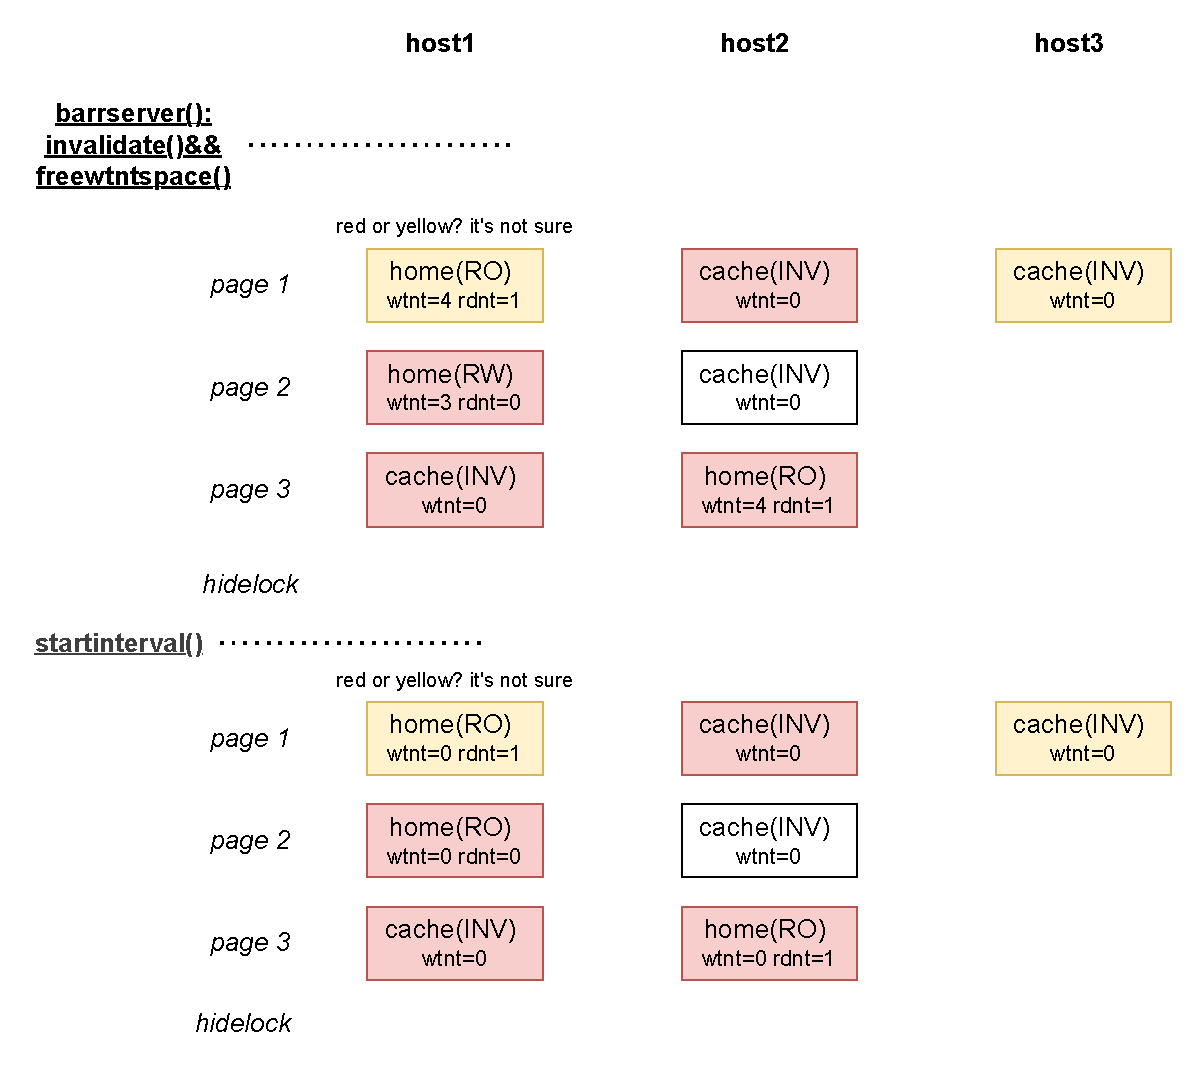
\includegraphics[width=0.8\textwidth]{Img/jiajia_barrier_sync2.drawio.pdf}
                  \bicaption{\enspace JIAJIA barrier同步操作}{\enspace JIAJIA barrier sync2}
                  \label{fig:JIAJIA-barrier2}
              \end{figure}
    \end{enumerate}

    % \begin{figure}[!htbp]
    %     \centering
    %     \begin{minipage}[t]{0.55\textwidth}
    %         \centering
    %         \includegraphics[width=\linewidth,page=1]{jiajia_barr_sync.drawio.pdf}
    %         \caption{barrier同步操作流程(1)}
    %     \end{minipage}
    %     \hfill
    %     \begin{minipage}[t]{0.55\textwidth}
    %         \centering
    %         \includegraphics[width=\linewidth,page=2]{jiajia_barr_sync.drawio.pdf}
    %         \caption{barrier同步操作流程(2)}
    %     \end{minipage}
    %     \bicaption{\enspace JIAJIA barrier同步操作}{\enspace JIAJIA lockstack layout}
    %     \label{fig:JIAJIA-barrier}
    % \end{figure}

    % \includepdf[pages=-,scale=0.8,pagecommand={\thispagestyle{fancy}}]{Img/jiajia_barr_sync.drawio.pdf}

    % \begin{figure}[!htbp]
    %     \centering
    %     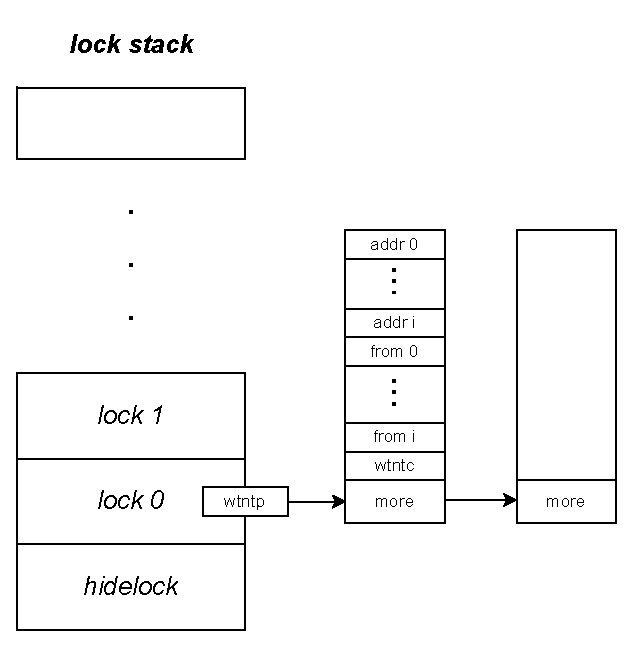
\includegraphics[width=0.6\textwidth]{Img/JIAJIA锁栈结构.drawio.pdf}
    %     \bicaption{\enspace JIAJIA 锁栈结构}{\enspace JIAJIA lockstack layout}
    %     \label{fig:JIAJIA-lockstack}
    % \end{figure}

    \section{本章小结}

    本章主要介绍了 JIAJIA 的关键技术,即设计架构和基于锁的一致性的实现。
}